\documentclass[numbers]{article}


% if you need to pass options to natbib, use, e.g.:
%     \PassOptionsToPackage{numbers, compress}{natbib}
% before loading neurips_2025


% ready for submission
% \usepackage{neurips_2025}


% to compile a preprint version, e.g., for submission to arXiv, add add the
% [preprint] option:
    \usepackage[preprint]{neurips_2025}


% to compile a camera-ready version, add the [final] option, e.g.:
%     \usepackage[final]{neurips_2025}


% to avoid loading the natbib package, add option nonatbib:
%    \usepackage[nonatbib]{neurips_2025}


\usepackage[utf8]{inputenc} % allow utf-8 input
\usepackage[T1]{fontenc}    % use 8-bit T1 fonts
\usepackage{hyperref}       % hyperlinks
\usepackage{url}            % simple URL typesetting
\usepackage{booktabs}       % professional-quality tables
\usepackage{amsfonts}       % blackboard math symbols
\usepackage{nicefrac}       % compact symbols for 1/2, etc.
\usepackage{microtype}      % microtypography
\usepackage{xcolor}         % colors
\usepackage{amsmath}
\usepackage{enumitem}
\usepackage[numbers]{natbib}
\usepackage{graphicx}
\usepackage{makecell}       % for \Xline

\title{FHGS}


% The \author macro works with any number of authors. There are two commands
% used to separate the names and addresses of multiple authors: \And and \AND.
%
% Using \And between authors leaves it to LaTeX to determine where to break the
% lines. Using \AND forces a line break at that point. So, if LaTeX puts 3 of 4
% authors names on the first line, and the last on the second line, try using
% \AND instead of \And before the third author name.


\author{%
  Q. G. Duan
  \thanks{Use footnote for providing further information about author (webpage, alternative address)---\emph{not} for acknowledging
    funding agencies.} \\
  Mechanical and Automation Erg\\
  Chinese University of Hong Kong\\
   % Shatin, N.T. 999077 \\
  \texttt{qigengduan@cuhk.edu.hk} \\
  % examples of more authors  
  \And
  Feihuang Xia \\
  BICMR\\
  Peking University\\
  \texttt{xiafeihuang@pku.edu.cn} \\
  \And
  Benyun Zhao \\
  Mechanical and Automation Erg\\
  Chinese University of Hong Kong\\
  %  Shatin, N.T. 999077 \\
  \texttt{byzhao@mae.cuhk.edu.hk} \\
  \And
  Mingqiao Han \\
  Mechanical and Automation Erg\\
  Chinese University of Hong Kong\\
   % Shatin, N.T. 999077 \\
  \texttt{mqhan@mae.cuhk.edu.hk} \\ 
  \And
  Yijun Huang \\
  Mechanical and Automation Erg\\
  Chinese University of Hong Kong\\
  %  Shatin, N.T. 999077 \\
  \texttt{yjhuang@link.cuhk.edu.hk} \\
  \And
  Ben M. Chen \\
  Mechanical and Automation Erg\\
  Chinese University of Hong Kong\\
  %  Shatin, N.T. 999077 \\
  \texttt{bmchen@cuhk.edu.hk} \\
  % \And
  % Coauthor \\
  % Affiliation \\
  % Address \\
  % \texttt{email} \\
}


\begin{document}


\maketitle


\begin{abstract}
  The abstract paragraph should be indented \nicefrac{1}{2}~inch (3~picas) on
  both the left- and right-hand margins. Use 10~point type, with a vertical
  spacing (leading) of 11~points.  The word Abstract} must be centered,
  bold, and in point size 12. Two line spaces precede the abstract. The abstract
  must be limited to one paragraph.
\end{abstract}


\section{Introduction}

In recent years, with the increasing demand for complex environmental interaction in unmanned systems, 3D scene understanding has gradually become a research focus. Traditional frameworks such as Multi-View Stereo (MVS) and Simultaneous Localization and Mapping (SLAM) can achieve geometric reconstruction, but exhibit limitations in high-level semantic perception and scene understanding. Recent advancements in Neural Radiance Fields (NeRF) and 3D Gaussian Splatting (3DGS) have introduced novel paradigms for 3D scene representation through differentiable frameworks:  NeRF models implicit radiance fields and learns continuous 3D spatial representations under 2D image supervision via differentiable volume rendering equations, while 3DGS employs explicit anisotropic GS primitives to achieve high-quality reconstruction through efficient rasterization. However, the ultimate objective of scene understanding requires not only precise geometric and appearance reconstruction, but also the integration of semantic features to achieve true scene "understanding" - a critical capability for autonomous decision-making and interactive tasks in unmanned systems.

%%这里加图:直观展示效果
\begin{figure}[htbp]
  \centering
  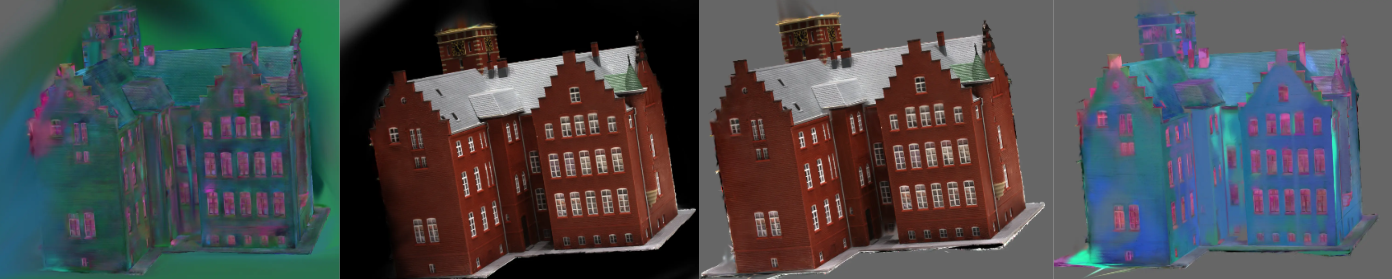
\includegraphics[width=0.8\textwidth]{start.png} % 替换为你的图片路径
  \caption{pipline of the xxxx}
  \label{fig:pipeline} % 标签名建议以 `fig:` 开头,方便区分
\end{figure}
To achieve this objective, 3D Scene Feature Field Fusion has emerged as a core research direction. Unlike traditional methods focusing solely on RGB fields, Feature Fields require maintaining semantic consistency across multiple viewpoints to avoid contradictory semantic predictions during viewpoint transitions, thereby enhancing global semantic reconstruction accuracy.
In this context, Feature Field fusion methods based on NeRF and 3DGS exhibit distinct characteristics:

NeRF-based framework extend feature fields by integrating learnable semantic feature fields into implicit radiance fields. While these methods implicitly encode multi-view semantic consistency through continuous neural representations, their inference speed is constrained by the dense sampling nature of volume rendering. Furthermore, geometric reconstruction quality and semantic feature fidelity often restrict each other.GS-based framework constructing explicit feature fields by directly associating semantic features with their explicit GS primitives. However, an inherent conflict arises between the anisotropic nature of RGB fields in their rasterization pipeline and the isotropic representation required for robust semantic features. Current methods typically enforce multi-view semantic consistency by directly reusing the rasterization framework of 3DGS. This approach inadvertently disrupts the self-attention relationships learned through architectures like Transformers, introducing noise during feature fusion and significantly degrading semantic rendering quality.

To address these challenges, we propose FHGS (Feature-Homogenized Gaussian Splatting), a Feature Fusion Method based on GS framework.Leveraging a differentiable framework, FHGS establishes bidirectional associations between 2D features and 3D feature fields, enabling end-to-end optimized multi-view consistent feature fusion. Crucially, FHGS retains the efficient and explicit representation of GS framework while overcoming the limitations of the Rasterization Method for RGB Fields. Specifically, each GS primitive is augmented with non-differentiable features, allowing the feature field to be directly supervised by feature ground-truth maps to enforce multi-view consistency.%In this way, the risk of destroying the stability of the geometric reconstruction by introducing complex differentiable features is avoided.

However, achieving multi-view feature consistency during rapid optimization while maintaining isotropic representation in the feature field remains a core challenge.  To address this, we innovatively introduce physics-inspired principles from electric field modeling, proposing a dual-drive mechanism:
\emph{External Potential Field Driving}: Treating feature ground-truth maps as electric fields, this mechanism directly guides the features of GS primitives to converge toward globally consistent semantic truth distributions.
\emph{Internal Feature Clustering Driving}: Leveraging feature discrepancies between GS primitives, this mechanism induces adaptive aggregation and repulsion in their spatial distribution, forming semantically coherent regional feature clusters that significantly suppress noise and accelerate external driving convergence.
By constraining anisotropy exclusively to photometric attributes while enforcing isotropy in features field driving, the method achieves global feature consistency optimization without modifying the intrinsic feature representation. Experiments demonstrate that the proposed mechanism not only enhances semantic fusion quality but also improves geometric reconstruction accuracy and noise robustness through feature-driven regularization effects.

The main contributions of this work are as follows:
\begin{itemize}
\item General Feature Fusion Architecture: We propose a GS-based feature field fusion framework capable of integrating 2D semantic features extracted from large-scale pre-trained models (e.g., SAM, CLIP), enabling unified optimization from low-level geometry to high-level semantics.
\item Integration of Non-Differentiable Features into GS Frameworks: Pioneering the integration of non-differentiable features into the differentiable 3DGS framework, this work fundamentally resolves the inherent contradiction between the anisotropic nature of Gaussian primitives and the isotropic requirements of semantic features.
\item Physics-Inspired Dual-Drive Mechanism: Drawing inspiration from electric field modeling, we design a joint optimization strategy combining external potential field driving and internal feature clustering driving, characterized by intuitive logic, computational efficiency, and strong interpretability.
\item Performance Superiority: On benchmark datasets (e.g., xxx, xxx), FHGS surpasses state-of-the-art methods (e.g., [Method-X]) by 4.2% in PSNR and 1.8 dB in reconstruction fidelity, while maintaining real-time rendering efficiency (≥60 FPS).
\end{itemize}

% 应用前景:
This work provides a novel technical pathway for 3D scene understanding in unmanned systems.  The efficient and robust feature fusion mechanism can be further extended to cutting-edge applications such as 3D dataset generation, dynamic scene modeling, and multimodal interaction.
%%这里加图:第二张图展示/gs椭球的各向异性,第三张图展示2DGS的几何同性
\begin{figure}[htbp]
  \centering
  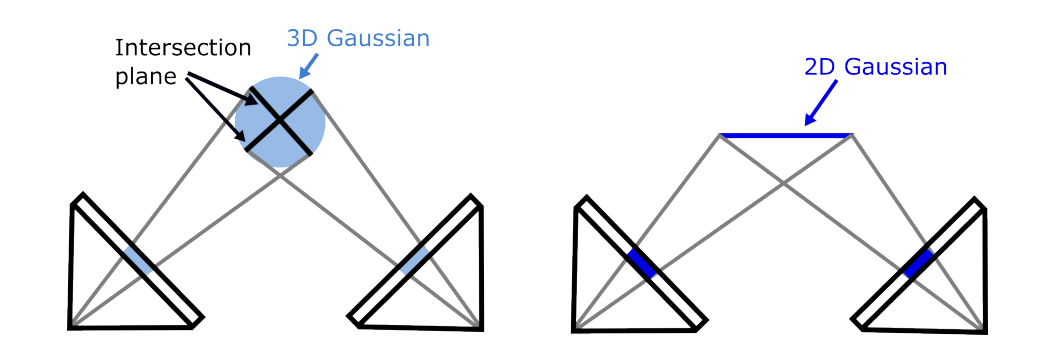
\includegraphics[width=0.8\textwidth]{2dgs.png} % 替换为你的图片路径
  \caption{pipline of the xxxx}
  \label{fig:pipeline} % 标签名建议以 `fig:` 开头,方便区分
\end{figure}

% ************ related work **************
\section{RELATED WORK}
\label{sec:related}
\subsection{Novel View Synthesis}
Neural Radiance Fields (NeRF)~\cite{nerf} introduced an implicit volumetric representation, where a continuous radiance field is modeled by multilayer perceptrons (MLPs). While delivering high-quality novel view synthesis, NeRF requires dense sampling and extensive computation during both training and inference. Solutions such as Mip-NeRF~\cite{mipnerf} and Mip-NeRF 360~\cite{mipnerf360} addressed sampling aliasing and unbounded scene reconstruction respectively, while Instant-NGP~\cite{instantngp} enabled real-time NeRF training by using hash-based encodings and fast optimization.

To overcome the inefficiencies of implicit representations, 3D Gaussian Splatting (3DGS)~\cite{3Dgaussians} reformulated scene modeling as a set of explicit anisotropic Gaussian ellipsoids in 3D space. Each ellipsoid encodes position, shape, orientation, and color attributes, enabling efficient and differentiable rasterization without neural networks. This approach supports real-time rendering and high-fidelity reconstruction, particularly benefiting from its explicit nature and rasterization pipeline.

Extending this idea, 2D Gaussian Splatting (2DGS)~\cite{2dgs} proposes a novel 2D Gaussian representation where each Gaussian is defined in the image plane and anchored to a 3D point, ensuring consistency across viewpoints. While achieving accurate appearance and geometry reconstruction, it faces limitations in handling semi-transparent surfaces and preserving fine geometry in texture-poor regions. To overcome this problem, our method \textit{FHGS} introduces high-level semantic priors from SAM, enabling structure-aware guidance during reconstruction.
% 使用了非可微分的信息(高维张量)来驱动语义分布的结构,使其更准确
Different from traditional Gaussian Splatting methods that rely purely on differentiable photometric cues, our \textit{FHGS} leverages non-differentiable, high-dimensional semantic information to guide the optimization of semantic-aware structural distributions, resulting in more precise and robust reconstructions, especially in challenging regions where appearance cues alone are insufficient.



\subsection{Implicit Feature Fusion}
Integrating semantic information or learned features into point-based scene representations is a well-established strategy, extensively explored in the NeRF literature~\cite{nerfsos,lerf,Dnerf,3dv,Inplace,P3su} and now migrating to Gaussian Splatting. Recent attemps to incorporate features into 2D/3D Gaussian Splatting can be clustered into three categories. Mask fusion approaches expemlified by GaussianCut~\cite{gaussiancut} and Gaussian Grouping~\cite{gaussian_grouping} project provided 2D masks onto the Gaussian set and employ graph-cut or low-dimensional identity embeddings for partitioning; While this method is straightforward for interactive 2D editing, the resulting correspondence is no longer perceptually obvious in 3D space, and the method still depends on extensive manual annotation while failing to capture any high-dimensional semantic features. External fusion schemes such as SAGA~\cite{saga}, Semantic Gaussians~\cite{semanticgaussian} and OmniSeg3D~\cite{omniseg3d} distil 2D features into 3D space through auxiliary neural network or contrastive learning, thereby enriching semantic information at the expense of additional parameters, prolonged training, and deviation from the concise design philosophy of Gaussian Splatting. Feature fusion techniques including Feature 3DGS~\cite{featureGS} and LangSplat~\cite{langsplat} associate learned embeddings with individual Gaussians so that semantics render with colour; however, these embeddings overwrite or reshape the high-dimensional tensors supplied by large segmentation models, erasing the self-attention structure and class relationships encoded therein and often introducing substantial noise that degrades segmentation quality; as a consequence, subsequent reasoning is confined to image space rather than the Gaussian domain. In contrast, we model cross-view semantic coherence as a physics-inspired potential-field optimization that relocates Gaussians while preserving their original feature vectors. The resulting procedure is self-supervised and globally consistent, retains the full high-dimensional semantic tensor for downstream tasks such as segmentation, detection and multi-modal prompting, and maintains the real-time rendering performance fundamental to Gaussian Splatting.


\section{METHODOLOGY}
This paper proposes FHGS (Feature-Homogenized Gaussian Splatting), a feature fusion method based on the GS framework that ensures multi-view consistency. FHGS addresses the semantic distortion and efficiency bottlenecks caused by the conflict between the anisotropic rendering mechanism of Gaussian Splatting and the isotropic requirements of high-level semantic features. As illustrated in Figure 2, the core components of FHGS include:
1.A general-purpose feature fusion architecture that supports the integration of multi-view features.
2.A GS framework enhanced with non-differentiable features, enabling the incorporation of high-dimensional semantic priors.
3.A dual-driven feature fusion mechanism inspired by physical modeling, which guides the feature optimization process using both geometric and semantic consistency cues.
\subsection{General Feature Fusion Architecture}
\begin{figure}[htbp]
  \centering
  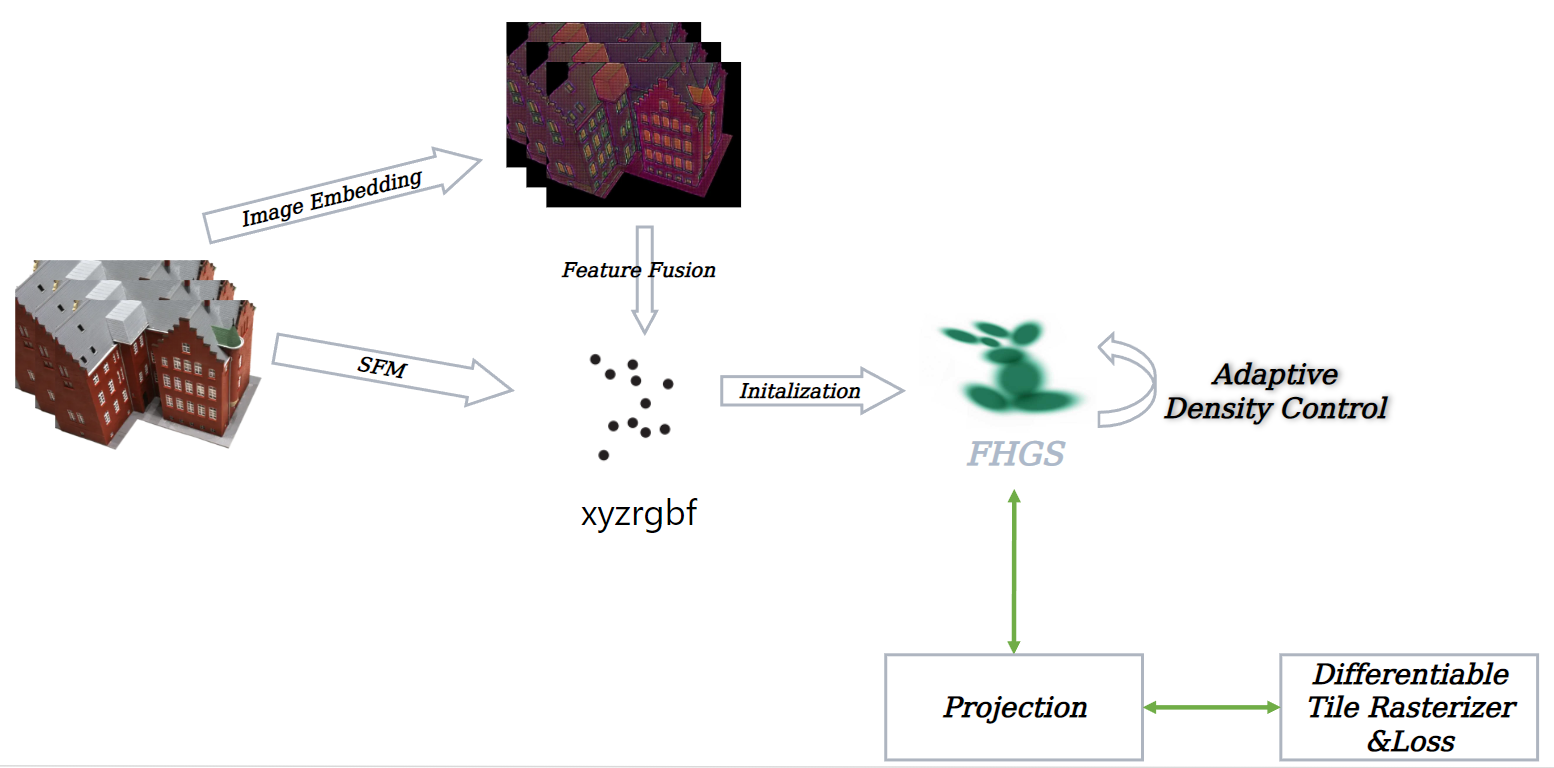
\includegraphics[width=0.8\textwidth]{featurepipeline.png} % 替换为你的图片路径
  \caption{pipline of the xxxx}
  \label{fig:pipeline} % 标签名建议以 `fig:` 开头,方便区分
\end{figure}

\subsection{Integration of Non-Differentiable Features into GS Frameworks}
2D Gaussian Splatting represents a scene as a collection of oriented elliptical disks whose densities and colours are composited in the image plane by tile-based $\alpha$-blending. These explicit primitives render in real time and remain fully differentiable, which makes them ideal carriers for high-dimensional semantic features. Each GS primitive is anchored at a centre \(p_i\) and endowed with two orthogonal tangent directions \(t_u,t_v\); the corresponding normal is \(t_w=t_u\times t_v\).  
Planar scales are denoted \(S=(s_u,s_v)\).  
Gathering geometry, appearance, opacity and a frozen feature vector, we write 
\begin{equation}
    \Theta_i=\{\,p_i,R_i,S_i,op_i,c_i,f_i\,\},
\end{equation}

where $3\times3$ matrix \(R_i=[t_u,t_v,t_w]\), $f_i$ is the non-differentiable feature obtained from the result of image embedding in SAM. All other symbols follow standard 3DGS notation. Any point \((u,v)\) in the tangent plane is mapped to world space by  

\begin{equation}
        P(u, v) = p_i + s_u t_u u + s_v t_v v = H(u, v, 1, 1)^\top
\end{equation}
with the homogeneous matrix \( H \in \mathbb{R}^{4 \times 4} \) factories translation, rotation and scale, defined as:

\begin{equation}
    \mathrm{H} =
        \begin{bmatrix}
          s_u t_u & s_v t_v & 0        & p_i \\
          0       & 0       & 0        & 1
        \end{bmatrix} = \begin{bmatrix}
          \text{RS} & p_i \\
          0         & 1
        \end{bmatrix}
\end{equation}

which factories rotation, scale and translation and thereby enables evaluation of densities directly in \(uv\)-space. Given local coordinates \(\mathbf u=(u,v)\), the unnormalized density is  

\begin{equation}
    \mathcal{G}(\mathbf{u}) = \exp(-\frac{u^2+v^2}{2})
\end{equation}

an isotropic Gaussian whose covariance is implicitly set by the $3\times3$ scale matrix \(S\). Then, let \(\mathbf{x}=(x,y)\) be a pixel and define \(\mathbf{u(x)}\) as the unique point in the splat's tangent plane whose homogeneous coordinates satisfy $\mathbf x=(xz,\;yz,\;z,\;z)^{\!\top}=WP(u,v)=WH(u,v,1,1)^{\!\top}$, where $W\in4\times4$ is the world to camera transform matrix, $H$ is the splat transform introduced above and $z$ is the depth. Ordered from back to front, the final color is obtained through: 
\begin{equation}
    \mathbf{c}(\mathbf{x}) 
    = \sum_{i=1}^{N} \mathbf{c}_i \, \mathbf{w}_i \
\end{equation}
 where the weight \(w_i = \alpha_i T_i\) as a dynamic differentiable parameter; while \(\alpha_i = op_i{\mathcal{G}}_i(\mathbf{u}(\mathbf{x}))\) characterizes the intrinsic properties of GS primitives, and  \(T_i = \prod_{j=1}^{i-1}(1-\alpha_j)\) encodes their transmittance. During the backward pass, gradients of\(w_i\) propagate through the chain rule to drive the optimization of the geometric parameters of Gaussian primitives; thereby enhancing scene reconstruction quality. As the pivotal variable bridging geometric representation and the differentiable rasterizer, \(w_i\) directly governs both reconstruction accuracy and rendering efficiency.
\begin{figure}[htbp]
  \centering
  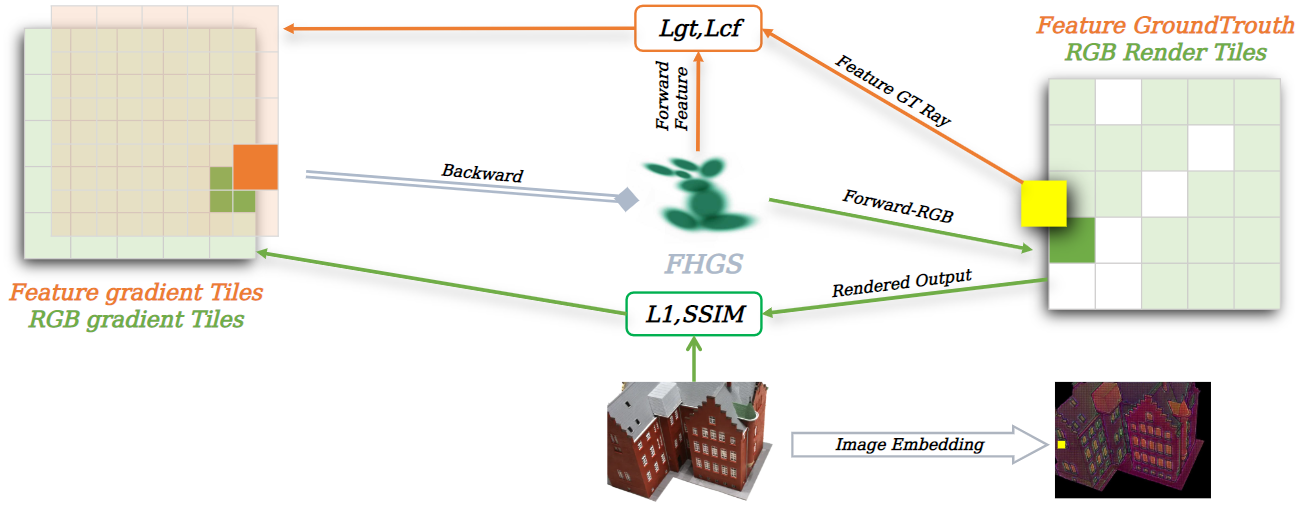
\includegraphics[width=0.8\textwidth]{nondiff.png} % 替换为你的图片路径
  \caption{pipline of the xxxx}
  \label{fig:pipeline} % 标签名建议以 `fig:` 开头,方便区分
\end{figure}
 We propose a GS framework with a non-differentiable feature fusion mechanism (orange pathway in Figure 4).During the forward process, the framework directly utilizes the pre-extracted Feature Ground-Truth Map
 \(F_{gt}\) to compute the feature loss \(L_{feat}\), which is formulated based on \(F_{gt}(p)\), the feature \(f_{i}\) of Gaussian primitives, and their contribution weights \(w_{i}\). In the backward process, gradients are propagated through \(w_{i}\) to to optimize the geometric parameters \(\{\,p_i,R_i,S_i,op_i\,\}\), implicitly driving the spatial distribution of Gaussian primitives toward feature-consistent regions.

 Compared to the differentiable rasterizer (green pathway in Figure 4), the non-differentiable branch eliminates the need for feature rendering during the forward process, enabling direct loss computation while preserving GS-Framework’s real-time performance. This design decouples conflicting objectives: the anisotropic color rendering remains dedicated to illumination and shadow modeling, while the multi-view consistency of non-differentiable features is achieved through \(w\) - driven distribution optimization, thereby avoiding direct conflicts between the rasterizer’s anisotropic mechanism and the isotropic requirements of semantic features.

\subsection{ Physics-Inspired Dual-Drive Mechanism}
% 本文提出的基于可微分渲染的三维重建优化框架,其核心方法建立在以下三个设计准则之上:(1) 继承SAM模型提取的不可微特征f_i,保持Transformer编码的单视图高维向量空间关系;(2) 利用跨视图语义相似性约束驱动几何基元分布;(3) 通过GS splatting自监督优化过程实现特征与几何的协同演化。

The core methodology of the 3D reconstruction optimization framework based on differentiable rendering proposed in this paper is established upon three design principles: (1) Inheriting the non-differentiable features \(f_i\) extracted by the SAM model while maintaining the high-dimensional vector space relationships of single-view Transformer encodings; (2) Utilizing cross-view semantic similarity constraints to drive the distribution of geometric primitives; (3) Achieving the co-evolution of features and geometry through a GS splatting self-supervised optimization process.
% 本方法受物理势场理论启发,将真值特征f_gt建模为具有特定性质的势场源,将高斯溅射基元(GS primitives)视为离散电荷体系,通过可微分光栅化实现势场梯度传播,最终驱动几何基元向能量最优位姿收敛。
Inspired by the theory of physical potential fields, This method models the ground-truth feature \(f_gt\) as a potential field source with specific properties, treats GS primitives as discrete charge systems, achieves potential field gradient propagation via differentiable rasterization, and ultimately drives geometric primitives to converge toward energy-optimal poses.
Building upon this theoretical framework, this study constructs a dual-potential-field-driven loss function system:

\begin{figure}[htbp]
  \centering
  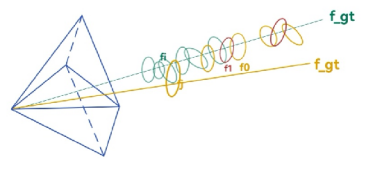
\includegraphics[width=0.8\textwidth]{dualdriveMe.png} % 替换为你的图片路径
  \caption{pipline of the xxxx}
  \label{fig:pipeline} % 标签名建议以 `fig:` 开头,方便区分
\end{figure}

% 外部势场约束: 在射线追踪的前向传播阶段,将每个像素看作射线,已知该射线l的feature为f_gt,则可计算射线路径上各GS基元特征f_i 与f_gt的余弦相似度,构建逐基元的辐射度损失:
\emph{External Potential Field Constraint}: During the forward propagation phase of ray tracing, by treating each pixel as a ray and leveraging the known feature \(f_{gt}\) of the ray\(l\), we compute the cosine similarity between the features \(f_i\) of Gaussian splatting primitives (GS primitives) along the ray\(l\) path and \(f_{gt}\), thereby constructing a per-primitive radiance loss:
\begin{equation}
    L_{gt} = \sum_{i=1}^{N} w_i \left(1 - f_{gt} \cdot f_i\right)
\end{equation}
%其中w_i表示基元i在射线l上的渲染权重公式为:xxx, 该公式中w_i可微分。反向传播时,通过w_i可以将梯度传播到GS基元内部的几何项,驱动椭球基元向语义匹配区域迁移。
%由于我们f_gt和f_i均作了归一化处理,所以cos<f_i,f_j>退化为f_idotf_j.
where \(w_i\) represents the rendering weight of primitive \(i\) for that pixel, \(w_i\) is derived from GS splatting using the formula:

In this formula,\( w_i\) is differentiable.  enabling gradient propagation to the geometric parameters within the GS primitives through \(w_i\) during backpropagation, thereby driving GS primitives to migrate toward semantically matched regions. Since both \(f_{gt}\) and \(f_i\) are normalized, the cosine similarity \(\cos\left\langle f_i, f_j \right\rangle\) reduces to \(f_i \cdot f_j\).

%内部势场优化:为建模GS基元间的特征一致性约束,本研究首先定义基于全局特征相似性的基础损失函数
\emph{Internal Potential Field Optimization}: To model the feature consistency constraints among GS primitives, this study first defines a foundational loss function based on global feature similarity.

\begin{align*}
    L_{cf} = \sum_{i=1}^{N}\sum_{j=1}^{N} w_i w_j\left(1 - \cos\left\langle f_i, f_j \right\rangle\right)
\end{align*}
%该式通过双重遍历计算所有GS基元对的加权余弦差异,旨在驱动相邻基元特征趋向一致。然而,直接应用此公式存在显著缺陷:(1) 计算复杂度为O(N2)难以满足实时性需求;(2) 全局遍历会引入跨物体基元间的无效排斥,破坏合法几何结构。针对上述问题,本研究提出层级累积式优化策略,将原始公式重构为线性复杂度形式:
This formulation computes the weighted cosine dissimilarity between all GS primitive pairs via dual iteration, aiming to drive neighboring primitive features toward consistency. However, directly applying this formula exhibits significant drawbacks: (1) The computational complexity of
\(O(N^2)\)is prohibitive for real-time requirements; (2) Global iteration introduces spurious repulsion between cross-object primitives, degrading valid geometric structures.
To address the aforementioned issues, this study proposes a hierarchical cumulative optimization strategy, reformulating the original formulation into a linear-complexity form \(O(N)\):

\begin{equation}
\begin{split}
    L_{cf} 
    &= \sum_{i=1}^{N}\sum_{j=1}^{i-1}\sigma_i w_i w_j\left(1 - f_j \cdot f_i\right) \\
    &= \sum_{i=1}^{N}\sigma_if(x)=\sigma_i w_i\left(\sum_{j=1}^{i-1}w_j - \sum_{j=1}^{i-1}w_j f_j \cdot f_i\right) \\
    &= \sum_{i=1}^{N}\sigma_i w_i\left(W_{i-1} - F_{i-1} \cdot f_i\right)
\end{split}
\end{equation}

%在反向传播钟,我们xxxx
\(\sigma_i = \frac{1}{1+e^{k(x-\lambda)}}\).

\begin{align*}
    \frac{\partial L_{gt}}{\partial w_k} = \sigma_k(W_{k-1}-F_{k-1}\cdot f_k) + \sum_{i=k+1}^{N}\sigma_i w_i(1 - f_i\cdot f_k)
\end{align*}

%表示前序基元的累积渲染权重
where\(W_n=\sum_{i=1}^{n}w_i\) represents the cumulative rendering weight of preceding primitives;
%为前序基元的加权特征均值
\(F_n=\sum_{i=1}^{n}w_i f_i\) represents the weighted feature mean of preceding primitives;
\(\sigma_i=Sigmoid\left( f_i \cdot f_{gt}\right)\) serves as the activation function.

%该方法利用率GSSplatting的渲染机制,创新性体现于三方面:(1)复杂度优化:通过沿射线传播由后到前的方向逐基元累积W_N和F_N,将计算复杂度从ON2降为0N,同时保留特征交互的物理意义。

%(2)激活函数调控:为避免优化初期因特征未对齐导致的过约束问题,引入基于全局相似度的激活函数:当GS基元i


%sigma_i基于全局相似度阈值激活,避免(3)遮挡感知机制:权重累积过程隐式建模渲染层级关系,仅对当前基元i与后序渲染基元(j<i)施加约束。理论推导证明,该优化公式与原始双重求和形式等价。






\label{sec:method}

\section{EXPERIMENTS}
\subsection{Comparative experiment}

\begin{table}[!htbp]
\centering
\caption{Ablation study}
\renewcommand{\arraystretch}{1.25}
\begin{tabular}{l | c c c}
\Xhline{1.2pt}
Metric & PSNR ($\pm$ s.d.)$\uparrow$  & SSIM ($\pm$ s.d.)$\uparrow$ & LPIPS ($\pm$ s.d.)$\uparrow$   \\
\hline
Ours (w/ speed-up) &  &  &  \\
Ours &  &  &   \\
3DGS (baseline) &  &  &  \\
\Xhline{1.2pt}
\end{tabular}
\label{tab:ablation1}
\end{table}


\subsection{Ablation Study}
\begin{figure}[htbp]
  \centering
  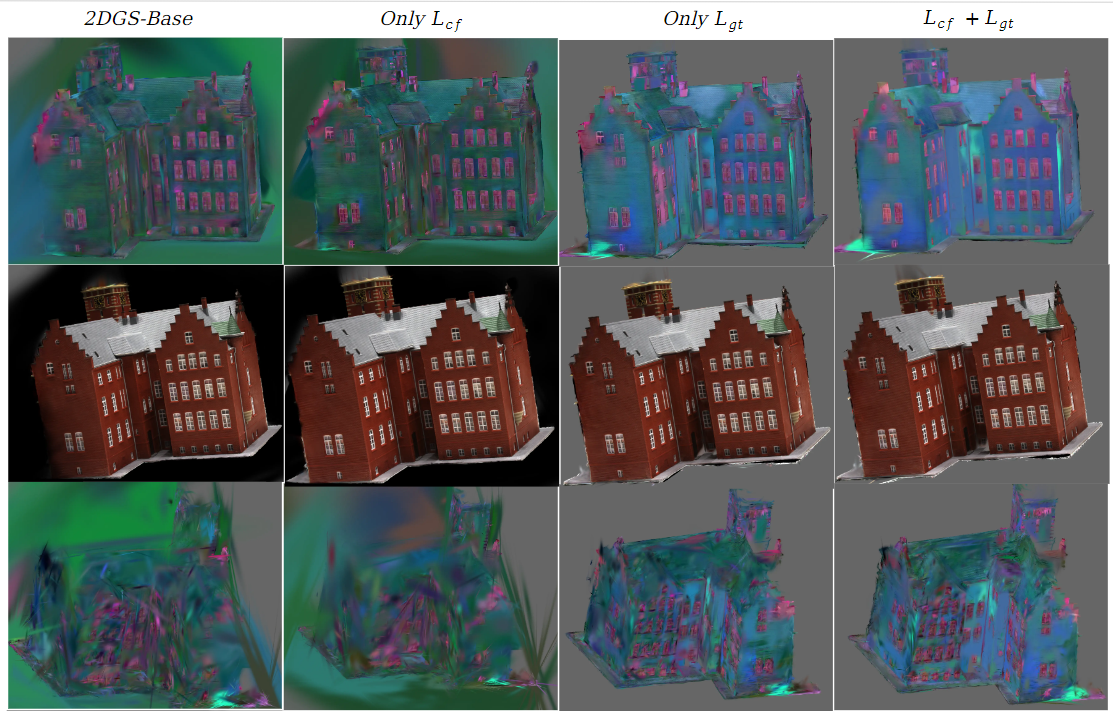
\includegraphics[width=0.8\textwidth]{ablationstudy.png} % 替换为你的图片路径
  \caption{pipline of the xxxx}
  \label{fig:pipeline} % 标签名建议以 `fig:` 开头,方便区分
\end{figure}
\begin{table}[!htbp]
\centering
\caption{Ablation study}
\renewcommand{\arraystretch}{1.25}
\begin{tabular}{l | c c c}
\Xhline{1.2pt}
Metric & mIoU $\uparrow$  & Accuracy $\uparrow$ & FPS $\uparrow$   \\
\hline
Ours (w/ speed-up) &  &  &  \\
Ours &  &  &   \\
\Xhline{1.2pt}
\end{tabular}
\label{tab:ablation2}
\end{table}


\begin{ack}
This study was supported by the InnoHK initiative of the Innovation and Technology Commission of the Hong Kong Special Administrative Region Government via the Hong Kong Centre for Logistics Robotics, and in part by the Research Grants Council of Hong Kong SAR under Grants 14206821, 14217922 and 14209623.
\end{ack}

\label{sec:exp}

\section{CONCLUSION}

\label{sec:exp}

\bibliographystyle{unsrtnat}   % or abbrvnat / plainnat / ieeetr, etc.
\bibliography{ref}      % name of the .bib file without extension



%%%%%%%%%%%%%%%%%%%%%%%%%%%%%%%%%%%%%%%%%%%%%%%%%%%%%%%%%%%%

\appendix

\section{Technical Appendices and Supplementary Material}
Technical appendices with additional results, figures, graphs and proofs may be submitted with the paper submission before the full submission deadline (see above), or as a separate PDF in the ZIP file below before the supplementary material deadline. There is no page limit for the technical appendices.

%%%%%%%%%%%%%%%%%%%%%%%%%%%%%%%%%%%%%%%%%%%%%%%%%%%%%%%%%%%%

\newpage
\section*{NeurIPS Paper Checklist}

%%% BEGIN INSTRUCTIONS %%%
The checklist is designed to encourage best practices for responsible machine learning research, addressing issues of reproducibility, transparency, research ethics, and societal impact. Do not remove the checklist: {\bf The papers not including the checklist will be desk rejected.} The checklist should follow the references and follow the (optional) supplemental material.  The checklist does NOT count towards the page
limit. 



\end{document}